\documentclass[12pt]{article}
\usepackage[english]{babel}
\usepackage[utf8x]{inputenc}
\usepackage[T1]{fontenc}
\usepackage{scribe}
\usepackage{listings}
\usepackage{fullpage}
\usepackage{amsfonts}
\usepackage{amssymb}
\usepackage{hyperref}
\usepackage{url}

\usepackage[svgnames]{xcolor}
\usepackage{color}
% \definecolor{light-gray}{gray}{0.90}
% \lstset{backgroundcolor=\color{light-gray},showlines=true}

% \usepackage{xcolor}
% \usepackage{listings}

% \lstdefinestyle{BashInputStyle}{
%   language=bash,
%   basicstyle=\small\sffamily,
%   numbers=left,
%   numberstyle=\tiny,
%   numbersep=3pt,
%   frame=tb,
%   columns=fullflexible,
%   backgroundcolor=\color{yellow!20},
%   linewidth=0.9\linewidth,
%   xleftmargin=0.1\linewidth
% }


\usepackage{minted}
\setminted{fontsize=\footnotesize,baselinestretch=0.5}


\Scribe{}
\Lecturer{Queenie Qiu, John Raiti. ~ Student: Fill in your name} 
\LectureNumber{2}
\LectureDate{DATE: Jan 19th. 2023}
\LectureTitle{Mapping \& Localization}

\lstset{style=mystyle}

\begin{document}
	\MakeScribeTop

%#############################################################
%#############################################################
%#############################################################
%#############################################################




 

\section {Navigation components}
Before we start we need to install some dependencies (if you are using ROS Kinetic, please change the following commands into kinetic):


\begin{minted}{bash}
$ sudo apt-get install ros-noetic-dynamixel-sdk
$ sudo apt-get install ros-noetic-turtlebot3-msgs
$ sudo apt-get install ros-noetic-turtlebot3
\end{minted}

We will use the turtlebot3\_world and the burger model for the turtlebot3. As a set up step, you can launch both the environment and the robot with the following command in a terminal:

\begin{minted}{bash}
  $ roslaunch turtlebot3_gazebo turtlebot3_world.launch
\end{minted}

It is important to select the turtlebot3 model before you launch the gazebo instance. Every terminal you open, you need to add the following command before running any ROS command related to the turtlebot3. In our present case it will be “burger”, but there are other models available, like the “waffle\_pi”.
\begin{minted}{bash}
  $ export TURTLEBOT3_MODEL=burger
\end{minted}

\textbf{Deliverable (review):} In the last lab, you may notice that you needed to run this command many times in new shells, but you can avoid that by adding this line to your .bashrc. What command can help you to do this?

Solution: 
\begin{minted}{bash}
  $ echo 'export TURTLEBOT3_MODEL=burger' >> ~/.bashrc
\end{minted}

Another tool that you may set up before we start this lab section, is the RViz visualization tool. RVIZ is a ROS graphical interface that allows you to visualize a lot of information, using plugins for many kinds of available topics. With the following command you will launch an RVIZ configuration which includes the turtlebot3 model and some of its most common topics

\begin{minted}{bash}
  $ roslaunch turtlebot3_gazebo turtlebot3_gazebo_rviz.launch
\end{minted}

Note: you may want to make changes to the RVIZ configuration. One strongly recommended, is to use “odom” as the Fixed frame. Currently, the robot has no map to refer to. That will change in the following subsections.

\subsection{Teleoperating the robot with the keyboard}
\begin{enumerate}
    

\item  First, we need to move the robot around and explore the simulated environment. We will use a teleoperation program that controls the robot by keyboard strokes, which will change the velocity values of the robot. In a new terminal launch the following:

\begin{minted}{bash}
  $ roslaunch turtlebot3_teleop turtlebot3_teleop_key.launch
\end{minted}

Now you are ready to explore how different keys make changes to linear and angular velocities.

\item  You can try to figure out what is happening by checking different topics. There are multiple options for rostopic command-line tool, for example:  list, echo, hz, pub. 

\textbf{Deliverable:} Describe what happens in the terminal when you execute the following command:

\begin{minted}{bash}
  $ rostopic echo /cmd_vel
\end{minted}

\textbf{Answer: }The command prints the data published on the topic \mintinline{bash}{/cmd_vel}.
\\Specifically, the command velocity of the robot, including its linear and angular velocities on axes \mintinline{bash}{x, y, z}, are published several times a second.

\item Move the robot around and observe how each key changes the velocity.

\begin{minted}[baselinestretch=1.2]{bash}
  w: linear vel +0.01, angular vel 0.0
  a: linear vel 0.0, angular vel +0.1
  s: linear vel 0.0, angular vel 0.0, reset
  d: linear vel 0.0, angular vel -0.1
  x: linear vel -0.01, angular vel 0.0
\end{minted}

\item  Another useful visualization tool allows you to gather information on the nodes that are active and how they are exchanging information through topics. rqt\_graph provides a GUI plugin for visualizing the ROS computation graph. In a new terminal run:
\begin{minted}{bash}
  $ rosrun rqt_graph rqt_graph
\end{minted}

\textbf{Deliverable:} 
\begin{enumerate}
    \item Take a screenshot of your resulting graph (By selecting Nodes/Topics (active), with the rostopic echo /cmd\_vel on).

    \begin{figure}[H]
      \centering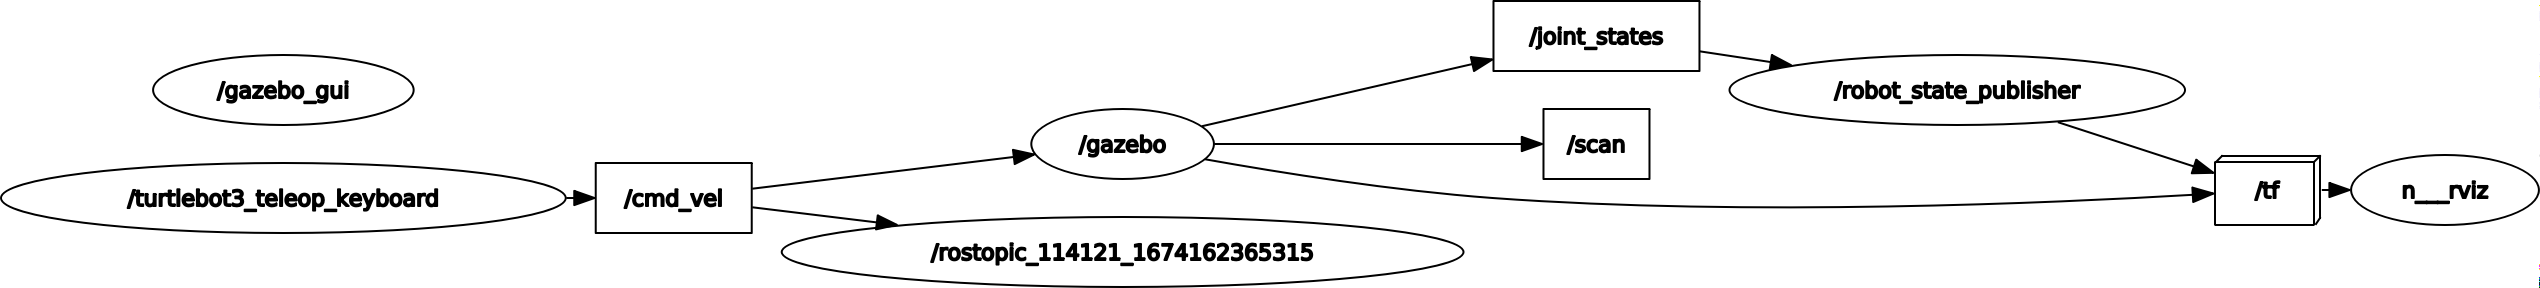
\includegraphics[width=14cm]{images/rosgraph_cmd_vel.png}\vspace{-10pt}
      \caption{Resulting graph with \mintinline{bash}{/cmd_vel} on.}\label{fig:cmd_vel}
      \end{figure}

    \item Please describe the graph. 
    
    \textbf{Answer: }On a high level, the user hits \mintinline{bash}{teleop} keys to control the robot, which utilizes and publishes joint information to calculate path to walk, rendered on RViz.
    \\Specifically:
    \begin{enumerate}
      \item Nodes \mintinline{bash}{/turtlebot3_teleop_keyboard} and \mintinline{bash}{/gazebo} communicate on the topic \mintinline{bash}{/cmd_vel}, i.e. command velocity. 
      \item Robot \mintinline{bash}{/gazebo} publishes information on the topic \mintinline{bash}{/scan} and communicates with the node \mintinline{bash}{/robot_state_publisher} with \mintinline{bash}{/join_states}, i.e. passive sensor.
      \item Nodes \mintinline{bash}{/gazebo} and \mintinline{bash}{/robot_state_publisher} both communicate with the renderer \mintinline{bash}{/n__rviz} on the topic \mintinline{bash}{/tf}.
    \end{enumerate}

\end{enumerate}

\end{enumerate}
\subsection{Creating a map}
The very first thing you need in order to perform navigation is a \textbf{map}: a representation of the environment where your robot will navigate. A map can be created from sensor readings of the robot. For example, a robot can estimate its own position by reading from odometry. At the same time the robot try to understand the positions of surrounding physical objects with data from sensors (for example, laser sensor or camera). These information allows robots to construct maps of the environment when the robots are moving around. The process is called Simultaneously Localization and Mapping (SLAM).  

\begin{enumerate}
    \item With the gazebo world launched (turtlebot3\_world) and the teleoperation program running (make sure to terminate the RViz terminal), execute the following command to launch the mapping component:
    \begin{minted}{bash}
  $ roslaunch turtlebot3_slam turtlebot3_slam.launch slam_methods:=gmapping
    \end{minted}
    This will use the gmapping method to acquire sensor readings and use SLAM to fuse the information and build the map of the robot’s surroundings as you move. You can visualize the results as you move using the newly launched RVIZ window.
    
    Note: If your gmapping does not work, it is highly likely the installation is not correct, we need to install:
    \begin{minted}{bash}
  $ sudo apt-get install ros-noetic-slam-gmapping
    \end{minted}
    \textbf{Deliverables:}
    \begin{enumerate}
    \item Take a screenshot of your resulting rqt\_graph (By selecting Nodes/Topics (active)).

    \begin{figure}[H]
      \centering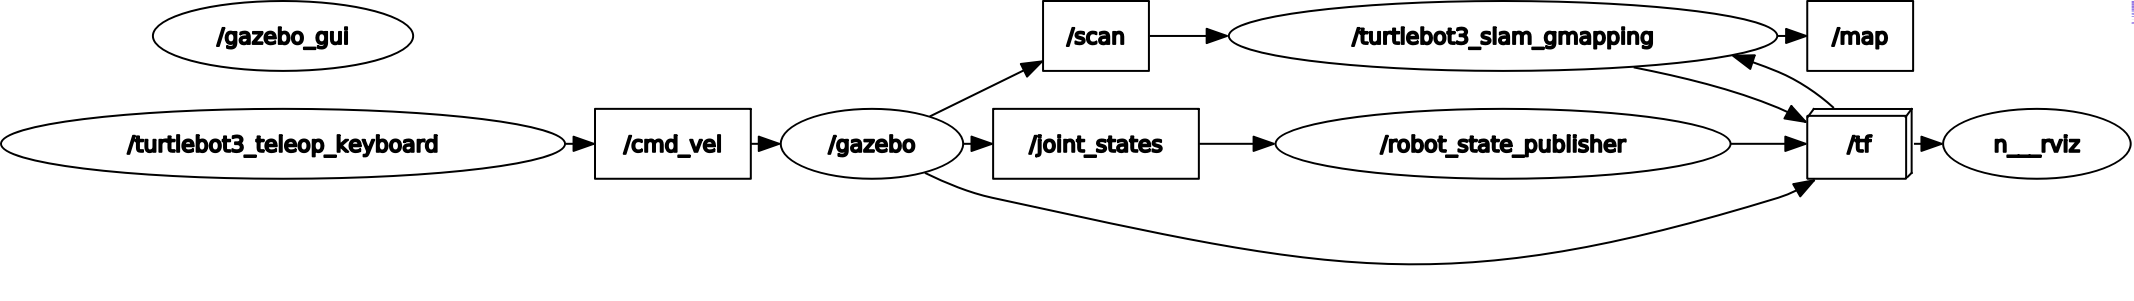
\includegraphics[width=14cm]{images/rosgraph_gmapping.png}\vspace{-10pt}
      \caption{Resulting graph with \mintinline{bash}{gmapping} working.}\label{fig:gmapping}
      \end{figure}

    \item Comparing with the rqt\_graph you got in the last deliverable, describe what changes for this rqt\_graph.  
\end{enumerate}

    \textbf{Answer: }The biggest difference between the two graphs is that \mintinline{bash}{/scan} with \mintinline{bash}{gmapping} connects to a new node, which then interconnects with an existing topic and leads to a new topic.
    \\Specifically, with \mintinline{bash}{gmapping} working, the robot is actively sensoring the surroudings, i.e. two nodes \mintinline{bash}{/gazebo} and \mintinline{bash}{/turtlebot3_slam_gmapping} are communicating on the topic \mintinline{bash}{/scan}.
    The traced space is output as text in the terminal, i.e. \mintinline{bash}{/turtlebot3_slam_gmapping} publishes map information on the topic \mintinline{bash}{/map}, and rendered on RViz, i.e. communicates with the node \mintinline{bash}{/n__rviz} on the topic \mintinline{bash}{/tf}.

        
    \item Teleoperate the robot around the room. When you have finished tracing the surroundings to complete the map, you can save it by running the following command in the terminal after finishing the gmapping launch.
    \begin{minted}{bash}
      $ rosrun map_server map_saver -f ~/map
    \end{minted}
     Note: This command will save the map in the current home directory. You may check this with ls commands. You may want to move the file to another containing folder, if you do some of the suggested commands in the next section will need to be adjusted accordingly. 
     
   \textbf{Deliverables:}
   You can inspect the output of your mapping in the .png and the .yaml files.
    \begin{enumerate}
        \item If there some holes between the gray and white parts of your map, can you state the reason? And how can you redo the map to have solid, thick, black lines? Note: You may have to run the mapping again and revisit those trouble areas with the teleoperation program.
        
        \textbf{Answer: }The holes inside the hexagon are in fact the borders of the white pillars.
        In order to generate solid black lines, the robot will have to move slowly and delicately around the pillars for SLAM to properly capture data from the surroundings, which can then be traced accurately.

        \item Take a screenshot of your final map.
        
        \begin{figure}[H]
          \centering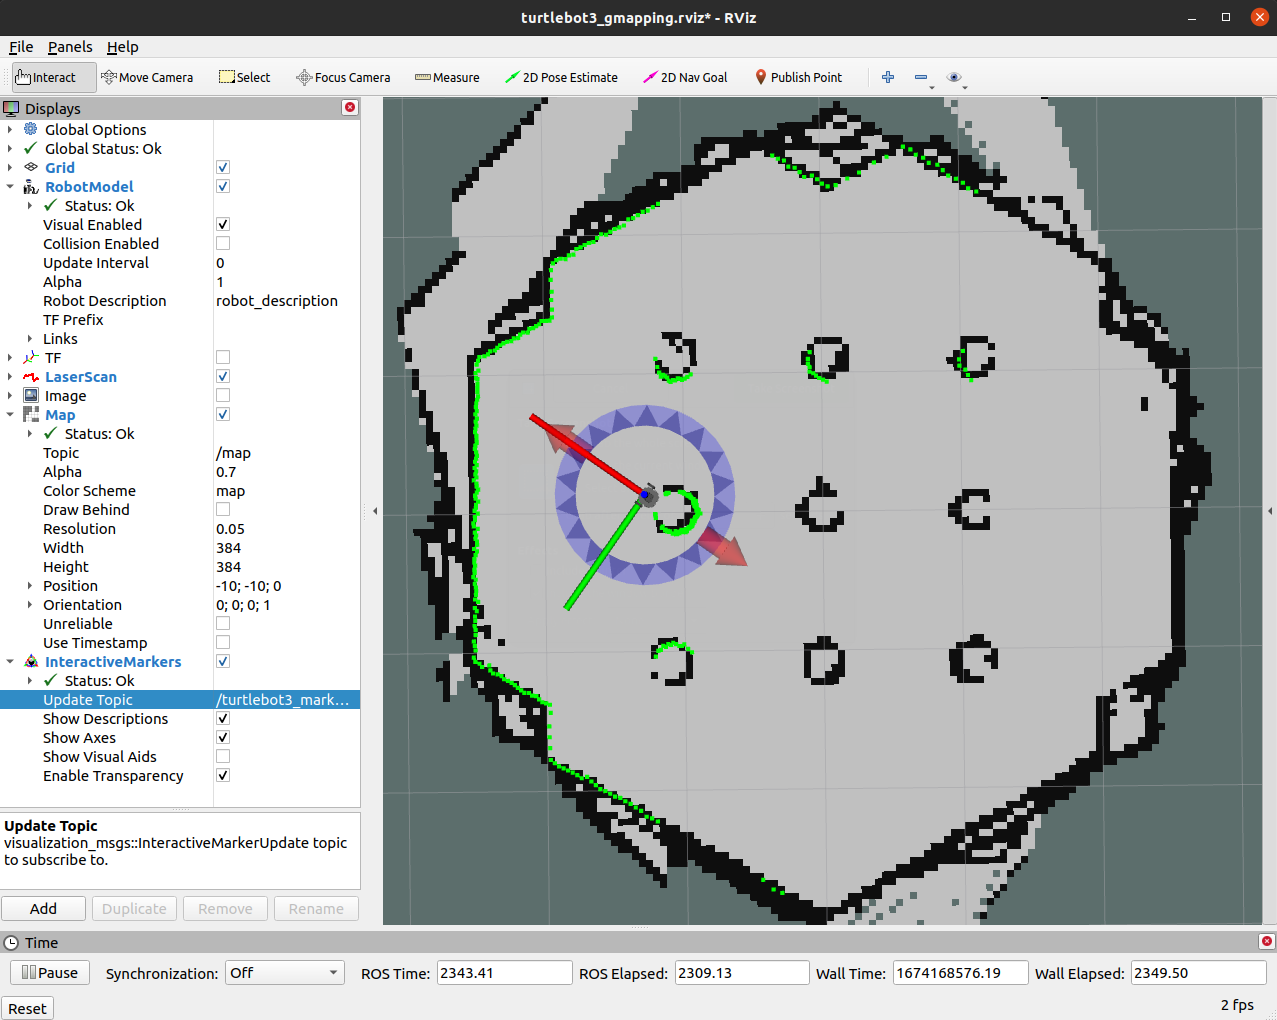
\includegraphics[width=14cm]{images/final_gmapping.png}\vspace{-10pt}
          \caption{Final map with \mintinline{bash}{gmapping} using InteractiveMarker.}\label{fig:final_gmapping}
          \end{figure}

        \item What is the ‘occupied threshold’ value?
        
        \textbf{Answer: }Pixels with occupancy probability greater than this threshold are considered completely occupied. It's \mintinline{bash}{0.65}.

        \item What is the ‘free threshold’ value?
        
        \textbf{Answer: }Pixels with occupancy probability less than this threshold are considered completely free. It's \mintinline{bash}{0.196}.
        
    \end{enumerate}
    
\end{enumerate}


\subsection{Navigating the map. 2D PoseEstimate and 2DNavGoal}

Robot navigation means the robot's ability to determine its own position in its frame of reference and then to plan a path towards some goal location. It means that 
once the robot gets a map, it need to establish its own position and orientation within the map (self-localization) in order to successfully navigate in the map. 

In this subsection we will address the localization estimation and how to navigate towards a goal in the map. Notice that this launch file requires a map file as the argument. We will provide the map that we just created.

The map that you created with gmapping is a static map. This means that the map won't be changed once you created it; it captures the environment as it is at the exact moment that the mapping process is being performed. During this assignment, we will also explore  what happens when the environment changes (by adding an obstacle) and how the navigation process needs to adapt its planning process dynamically.

\begin{enumerate}
    \item Still working with the turtlebot3\_world and the teleoperation program (make sure to close the RViz window it will be relaunched), we will launch a navigation file:
     \begin{minted}{bash}
    $ roslaunch turtlebot3_navigation turtlebot3_navigation.launch map_file:=
    $HOME/map.yaml
         \end{minted}
         
    Note: If it didn't work, it is highly likely we need to install dependencies:
    \begin{minted}{bash}
    sudo apt-get install ros-noetic-dwa-local-planner
    \end{minted}
    Start moving the Robot around the room using the keyboard teleop. As you move the robot around, the green arrows represent location guesses of the robot in the map. That is, the localization algorithm calculate possible positions of the robot. The arrows will converge to the most likely location when you move the robot.
    
    \textbf{Deliverables:}
    Inspect the RViz components, different types of maps/costmaps and the topics associated with each component.
    
    \begin{enumerate}
        \item Does sensor measurement align well with the static map you created in section 1.2?
        
        \textbf{Answer: }It doesn't align as well as I expected it to be.
        
    \end{enumerate}
    \item You can help the robot localize by re-initializing its location on the map. To do that, go to the RVIZ window. Then press the button 2DPoseEstimate, go to the map, drop at the robot's location and drag the arrow in the robot's orientation (by visual approximation). The green arrows will be spread around that location. Notice how, before you provide the 2DPoseEstimate, the uniformity in shape of the turtlebot3\_world affects the localization estimate.
    
    \textbf{Deliverables:}
    \begin{enumerate}
        \item Take a screenshot of when there is a good alignment.
        
        \begin{figure}[H]
          \centering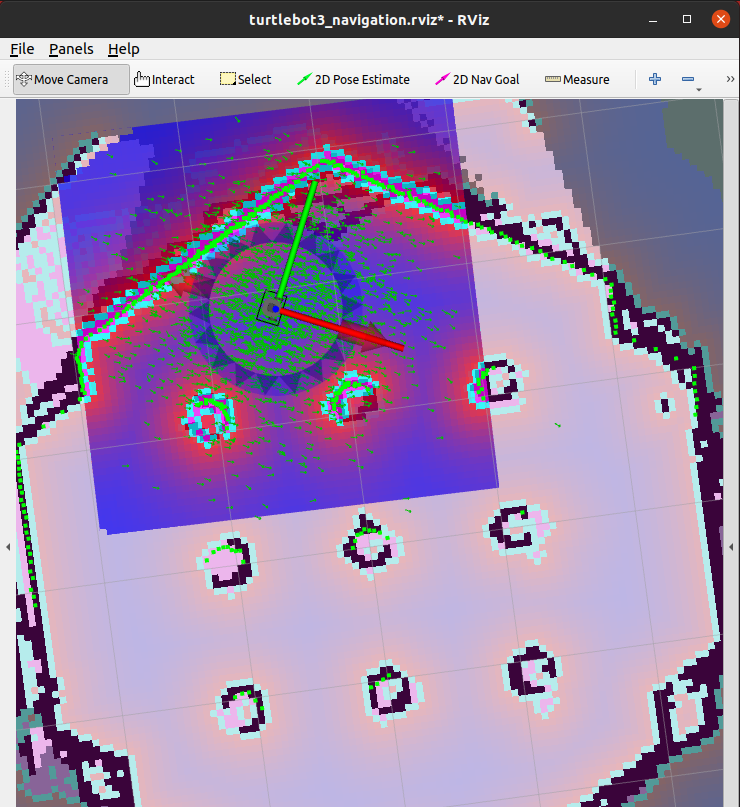
\includegraphics[width=14cm]{images/good_alignment.png}\vspace{-10pt}
          \caption{Optimizing sensor measurement alignment with \mintinline{bash}{2DPoseEstimate}.}\label{fig:good_alignment}
          \end{figure}

        \item As you teleoperate your robot using the teleop\_key, describe what is happening to the green arrows (It might show as green dots, but actually they are arrows) and the reason why the green arrows have that phenomenon. 
        
        \textbf{Answer: }The green arrows move in the same direction in which the robot moves, and they accumulate as the robot moves faster. It is assumed that the arrows represent the velocity of the robot, which is why them as a whole indicates the direction and magnitude of the velocity of the robotic patrol.

    \end{enumerate}
    
    \item Another feature in the RViz GUI, is the option to send Navigation goals to the robot. At this point, the teleoperation program needs to be terminated. You can command the robot by pressing the button 2DNavGoal and clicking on the map where an arrow will appear and release the mouse to provide the orientation. You can observe the planned trajectory and the robot moving towards this new location.\\
    Note: You need to terminate the teleop\_key such that the navigation can start. 
    
    \textbf{Deliverables:}
    \begin{enumerate}
        \item Describe the robot behaviors from the moment a navigation goal is given to the moment when the robot reaches its destination. Did the robot find any difficulties planning the route?
        
        \textbf{Answer: }When planning the path, the robot first twirls around to adjust its orientation, facing the path, and then moves along the path dynamically, avoids the red grids, and adjusts its orientation again before settling in the destination.
        \\When the starting or ending point happens to be around the edges of unavailable spots, the robot has difficulty planning the route and adjusts its direction.

        \item Check the map.yaml file for costmaps thresholds (free/occupied threshold) and try to understand them and grid occupancy. Determine if the robot goes closer or farther away from the map edges as it plans its movements.
        
        \textbf{Answer: }As stated before, pixels with occupancy probability greater than the occupied threshold are considered completely occupied, and less than the free threshold are considered completely free.
        \\When the robot is moving, it moves further away from the edges of the occupied grids (obstables, map) and closer to the free ones.

        \item What do the colors(red/blue) in the costmaps mean?
        
        \textbf{Answer: }The red grids in the costmap indicate edges of the occupied grids, including obstacles and other kinds of unavailable destinations.
        \\The blue grids in the costmap indicate a space in which the robot is free to move. It is a symbolic square-shaped area around the robot and a subset of a larger empty space.

    \end{enumerate}
    
    \item Another way to provide navigation goals is by publishing directly into the goal topic:
    \begin{minted}{bash}
    $ rostopic pub /move_base_simple/goal geometry_msgs/PoseStamped '
    {header: {stamp: now, frame_id: "map"}, pose
    : {position: {x: <value>, y: <value>, z: <value>}, orientation: {w: <value>}}}'
    \end{minted}
    
    
    \item Now add an obstacle (insert the pillar you previously created)
    You now have both static obstacles and a dynamic (new) obstacle that isn’t part of your map. 
    
    \textbf{Deliverables:}
    \begin{enumerate}
        \item Describe the robot behaviors from the moment a navigation goal is given to the moment when the robot reaches its destination. Did the robot find any difficulties planning the route?
        
        \textbf{Answer: }As described in 1.3.3.(a), the robot first plans the route, rotates its orientation, walks the path, avoids the obstacles, reaches the destination and adjusts its orientation.
        \\However, with the new dynamic obstable added, it encountered difficulties when planning a route that involves the new pillar. It would keep trying to replan the route with its sensor measurements before reporting errors and stopping.
        \\The same happens when it starts or ends at the edges of obstacles, which makes it repeatedly replan routes before declaring failure.

        \item Compare the local costmap/global costmap to the static map in RViz. What happens to the laser readings that you visualize?
        
        \textbf{Answer: }When approaching the dynamic obstable, a newly added pillar, its edges can be detected by the laser and displayed in the costmap as green. But since it isn't recorded in the static map, there isn't a black line indicating its shape.
        \\The green edges of the pillar would disappear when moving away and the pillar being out of the blue area, since the obstacles can be sensored by the LiDAR anymore, decreasing the readings to zero.
        
        \item Take a snapshot of the resulting rqt\_graph when running the navigation portion, and highlight the nodes actively participating in moving the robot from point A to B. Comment on the type of messages being shared on which topics and the direction of communication (who is a publisher and who is a subscriber to which topic).
        
        \begin{figure}[H]
          \centering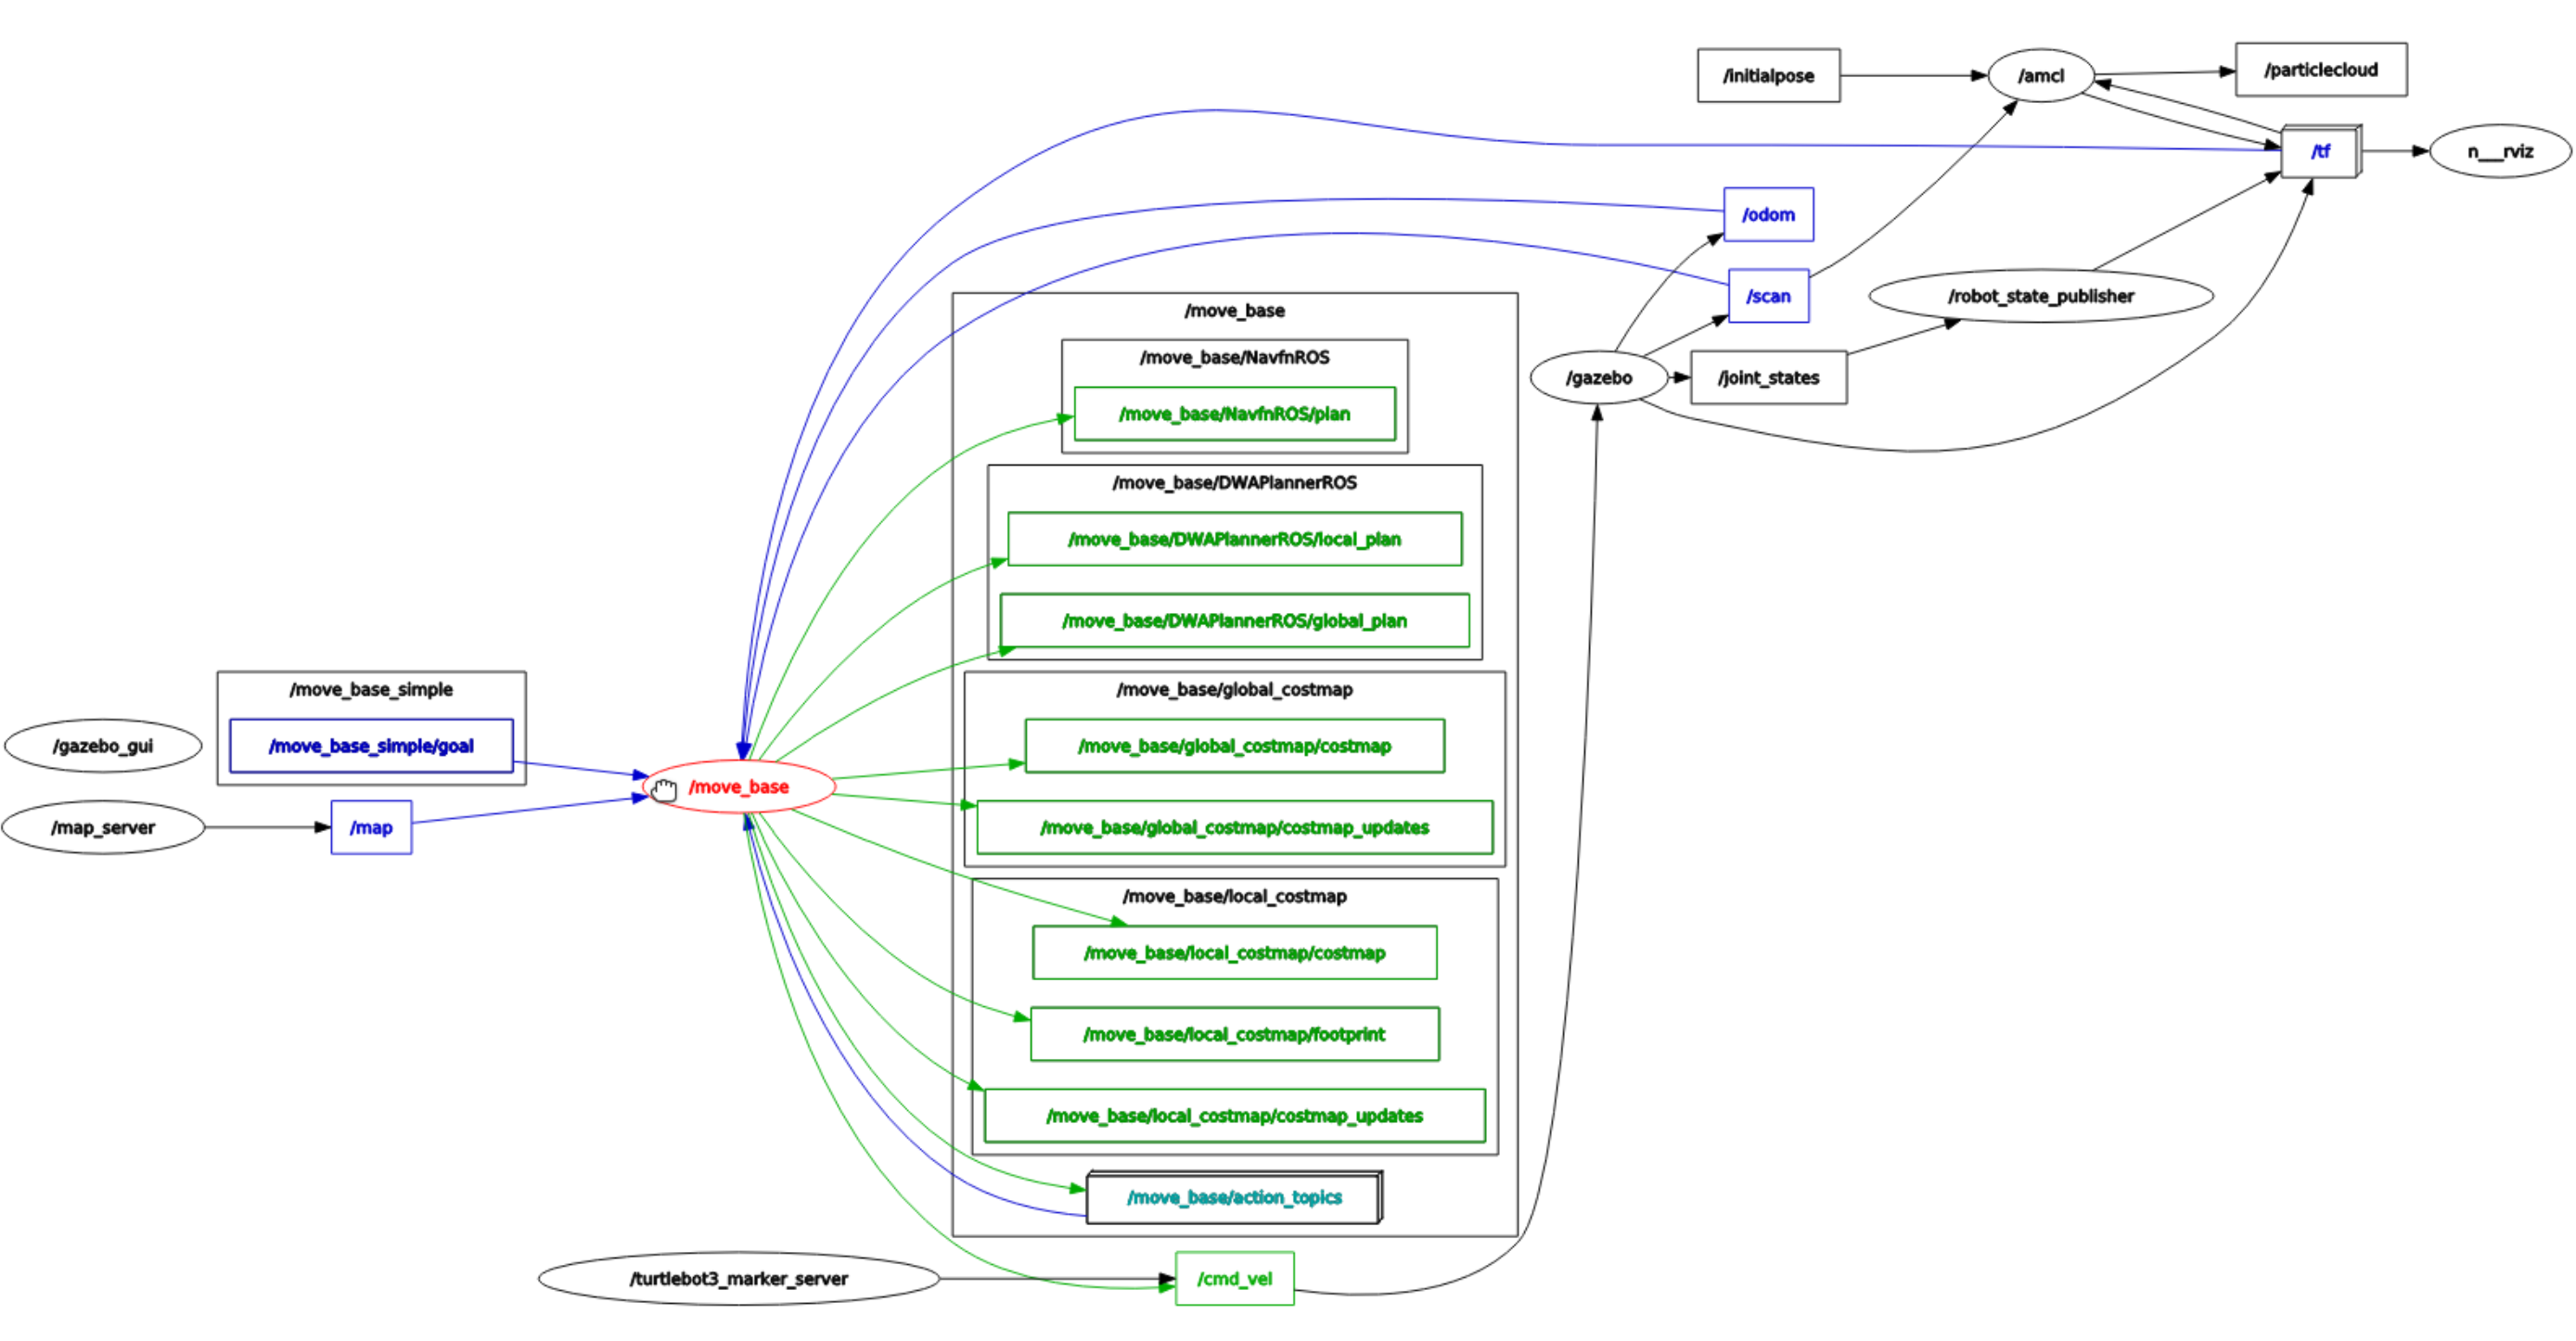
\includegraphics[width=14cm]{images/navigation_rqt_graph.png}\vspace{-10pt}
          \caption{Resulting \mintinline{bash}{rqt_graph} when running the navigation feature.}\label{fig:navigation_graph}
          \end{figure}
        
        \item Upload a video that shows the robot navigating to a new location using 2DNav Goal without the pillar.
        \item Upload a video that shows the robot navigating to a new location using 2DNav Goal that avoids the pillar that you inserted.
        
        Note: You can upload your videos into the google drive and share a link. Please put your link below:
        
        \href{https://drive.google.com/drive/folders/1zuAvhevD33JzZjYobt6tLiEW6jaDhEhm?usp=sharing}{Google Drive link to the videos.}

    \end{enumerate}

\end{enumerate}

\end{document}